\fuxiti
\begin{xiaotis}
\begin{enhancedline}

\xiaoti{半径为 $r$ 的圆的弦长为 $l$, 弦心距为 $d$, 弓形高为 $h$。}
\begin{xiaoxiaotis}

    \xxt{用 $r$ 和 $d$ 表示 $l^2$;}

    \xxt{用 $r$ 和 $h$ 表示 $l^2$。}
\end{xiaoxiaotis}

\xiaoti{以等边三角形的一边为直径作圆。求证:这圆平分其他两边,其他两边三等分半圆。}

\xiaoti{如图, $\yuanhu{AC} = \yuanhu{CB}$, $D$、$E$ 分別是 $OA$ 和 $OB$ 的中点。
    求证: $DC = CE$。
}

\begin{figure}[htbp]
    \centering
    \begin{tikzpicture}
    \pgfmathsetmacro{\R}{1.5}

    \tkzDefPoints{0/0/O}
    \tkzDefPoint(170:\R){A}
    \tkzDefPoint(110:\R){C}
    \tkzDefPoint(50:\R){B}
    \tkzDefMidPoint(O,A)  \tkzGetPoint{D}
    \tkzDefMidPoint(O,B)  \tkzGetPoint{E}

    \tkzDrawCircle[thick](O,A)
    \tkzDrawSegments(O,A  O,B  C,D  C,E)

    \tkzLabelPoints[below](O)
    \tkzAutoLabelPoints[center=O, centered, dist= .2](A,B,C)
    \tkzLabelPoints[below](D)
    \tkzLabelPoints[right](E)
\end{tikzpicture}


    \caption*{(第 3 题)}
\end{figure}

\xiaoti{$\triangle ABC$ 的高 $AD$、$BE$ 相交于点 $H$, $AD$ 的延长线交外接圆于点 $G$。
    求证: $D$ 为 $HG$ 的中点。
}

\xiaoti{$\triangle ABC$ 中, $BC = 2.4$ cm, $\angle A = 31^\circ$,利用三角函数表计算
    $\triangle ABC$ 的外接圆直径(精确到 0.1 cm)。
}

\xiaoti{$\triangle ABC$ 中, $BC = a$、 $CA = b$、 $AB = c$, 外接圆半径为 $R$。
    求证: $\dfrac{a}{\sin A} = \dfrac{b}{\sin B} = \dfrac{c}{\sin C} = 2 R$。
}

\begin{figure}[htbp]
    \centering
    \begin{minipage}[b]{4.5cm}
        \begin{tikzpicture}
    \pgfmathsetmacro{\R}{1.5}

    \tkzDefPoints{0/0/O}
    \tkzDefPoint(70:\R){A}
    \tkzDefPoint(210:\R){B}
    \tkzDefPoint(330:\R){C}
    \tkzDefPoint(150:\R){D} % CD 为直径

    \tkzDrawCircle[thick](O,A)
    \tkzDrawPolygon(A,B,C)
    \tkzDrawSegments[dashed](B,D  C,D)
    \tkzDrawPoint(O)

    \tkzMarkAngle[size=.4](B,A,C)
    \tkzMarkAngle[size=.4](B,D,C)
    \tkzLabelSegment[below](B,C){$a$}
    \tkzLabelPoints[above](O)
    \tkzAutoLabelPoints[center=O, centered, dist= .2](A,B,C)
\end{tikzpicture}


    \end{minipage}
    \begin{minipage}[b]{4.5cm}
        \begin{tikzpicture}
    \pgfmathsetmacro{\R}{1.5}

    \tkzDefPoints{0/0/O}
    \tkzDefPoint(70:\R){A}
    \tkzDefPoint(180:\R){B}
    \tkzDefPoint(0:\R){C}

    \tkzDrawCircle[thick](O,A)
    \tkzDrawPolygon(A,B,C)
    \tkzDrawPoint(O)

    \tkzMarkRightAngle[size=.2](B,A,C)
    \tkzLabelSegment[pos=.6, below](B,C){$a$}
    \tkzLabelPoints[above](O)
    \tkzAutoLabelPoints[center=O, centered, dist= .2](A,B,C)
\end{tikzpicture}


    \end{minipage}
    \begin{minipage}[b]{4.5cm}
        \begin{tikzpicture}
    \pgfmathsetmacro{\R}{1.5}

    \tkzDefPoints{0/0/O}
    \tkzDefPoint(70:\R){A}
    \tkzDefPoint(150:\R){B}
    \tkzDefPoint(30:\R){C}
    \tkzDefPoint(330:\R){D} % BD 为直径

    \tkzDrawCircle[thick](O,A)
    \tkzDrawPolygon(A,B,C)
    \tkzDrawSegments[dashed](B,D  C,D)
    \tkzDrawPoint(O)

    \tkzMarkAngle[size=.2](B,A,C)
    \tkzMarkAngle[size=.4, arc=ll](C,D,B)
    \tkzLabelSegment[pos=.7, below](B,C){$a$}
    \tkzLabelPoints[below](O)
    \tkzAutoLabelPoints[center=O, centered, dist= .2](A,B,C)
\end{tikzpicture}


    \end{minipage}
    \caption*{(第 6 题)}
\end{figure}

\xiaoti{已知: $a$、$b$、$c$ 为 $\triangle ABC$ 三边的长, $R$ 为其外接圆的半径。
    利用 $\dfrac{a}{\sin A} = \dfrac{b}{\sin B} = \dfrac{c}{\sin C} = 2 R$ 证明:
    $$ S_{\triangle ABC} = 2 R^2 \sin A  \sin B \sin C = \dfrac{abc}{4R} \juhao $$
}

\xiaoti{内接于圆的四边形 $ABCD$ 的对角线 $AC$ 与 $BD$ 垂直相交于点 $K$,
    过点 $K$ 的直线与边 $AD$、$BC$ 分别相交于点 $H$ 和 $M$。求证:
}
\begin{xiaoxiaotis}

    \xxt{如果 $KH \perp AD$, 那么 $CM = MB$;}

    \xxt{如果 $CM = MB$, 那么 $KH \perp AD$。}
\end{xiaoxiaotis}

\xiaoti{求证:四边形各内角的平分线所成的四边形内接于圆。}

\xiaoti{如图,延长圆的内接四边形 $ABCD$ 的两组对边,分别相交于点 $M$、$N$。
    求证:所成的 $\angle AMD$ 和 $\angle ANB$ 的平分线互相垂直。
    (提示:证明图中 $\angle 1 = \angle 2$。)
}

\begin{figure}[htbp]
    \centering
    \begin{minipage}[b]{7.5cm}
        \centering
        \begin{tikzpicture}
    \pgfmathsetmacro{\R}{1.5}

    \tkzDefPoints{0/0/O}
    \tkzDefPoint(120:\R){A}
    \tkzDefPoint(260:\R){B}
    \tkzDefPoint(310:\R){C}
    \tkzDefPoint(25:\R){D}
    \tkzInterLL(A,B)(D,C)  \tkzGetPoint{M}
    \tkzInterLL(A,D)(B,C)  \tkzGetPoint{N}
    \tkzDefLine[bisector](D,M,A)  \tkzGetPoint{h}
    \tkzDefLine[bisector](A,N,B)  \tkzGetPoint{e}
    \tkzInterLL(N,e)(A,B)  \tkzGetPoint{E}
    \tkzInterLL(N,e)(C,D)  \tkzGetPoint{G}
    \tkzInterLL(M,h)(A,D)  \tkzGetPoint{H}
    \tkzInterLL(M,H)(B,C)  \tkzGetPoint{F}
    \tkzInterLL(M,H)(N,E)  \tkzGetPoint{K}

    \tkzDrawCircle[thick](O,A)
    \tkzDrawPolygons(A,M,D  A,B,N)
    \tkzDrawSegments(M,H  N,E)

    \extkzLabelAngel[0.3](M,E,N){$1$}
    \extkzLabelAngel[0.3](E,G,M){$2$}
    \tkzAutoLabelPoints[center=O, centered, dist= .2](A,C,D)
    \tkzLabelPoints[below, xshift=-.5em](B)
    \tkzLabelPoints[below](M)
    \tkzLabelPoints[right](N)
    \tkzLabelPoints[left](E)
    \tkzLabelPoints[above, xshift=.4em](F)
    \tkzLabelPoints[above, xshift=-.5em](G)
    \tkzLabelPoints[above](H)
    \tkzLabelPoints[above, xshift=-.5em](K)
\end{tikzpicture}


        \caption*{(第 10 题)}
    \end{minipage}
    \qquad
    \begin{minipage}[b]{7cm}
        \centering
        \begin{tikzpicture}
    \tkzDefPoints{0/0/A, 1.5/0/B, 1.2/1/C}
    \tkzDefPointOnLine[pos=2.0](A,B)  \tkzGetPoint{D}
    \tkzDefPointOnLine[pos=2.0](A,C)  \tkzGetPoint{E}
    \tkzDefPointOnLine[pos=2.8](B,C)  \tkzGetPoint{F}
    \tkzDefPointOnLine[pos=2.3](B,A)  \tkzGetPoint{G}
    \tkzDefPointOnLine[pos=2.3](C,A)  \tkzGetPoint{H}
    \tkzDefPointOnLine[pos=2.8](C,B)  \tkzGetPoint{K}
    \tkzDrawSegments(D,G  E,H  F,K)
    \tkzLabelPoints[left=1em, yshift=-.5em](A)
    \tkzLabelPoints[right, yshift=-.5em](B)
    \tkzLabelPoints[above=.2em, xshift=.3em](C)
    % \tkzLabelPoints[](D,...,H,K)

    \tkzDefCircle[in](A,B,C)  \tkzGetPoints{I}{R}
    \tkzDrawCircle[thick](I,R)

    \tkzDefLine[bisector](D,B,C)  \tkzGetPoint{x}
    \tkzDefLine[bisector](B,C,E)  \tkzGetPoint{y}
    \tkzInterLL(B,x)(C,y)  \tkzGetPoint{I_a}
    \tkzDefLine[altitude](B,I_a,C)  \tkzGetPoint{R_a}
    \tkzDrawCircle[thick](I_a,R_a)

    \tkzDefLine[bisector](F,C,A)  \tkzGetPoint{x}
    \tkzDefLine[bisector](C,A,G)  \tkzGetPoint{y}
    \tkzInterLL(C,x)(A,y)  \tkzGetPoint{I_b}
    \tkzDefLine[altitude](C,I_b,A)  \tkzGetPoint{R_b}
    \tkzDrawCircle[thick](I_b,R_b)

    \tkzDefLine[bisector](H,A,B)  \tkzGetPoint{x}
    \tkzDefLine[bisector](A,B,K)  \tkzGetPoint{y}
    \tkzInterLL(A,x)(B,y)  \tkzGetPoint{I_c}
    \tkzDefLine[altitude](A,I_c,B)  \tkzGetPoint{R_c}
    \tkzDrawCircle[thick](I_c,R_c)

    \tkzDrawPoints(I, I_a, I_b, I_c)
    \tkzLabelPoints[right=-.2em](I)
    \tkzLabelPoints[right](I_a, I_b, I_c)
\end{tikzpicture}


        \caption*{(第 14 题)}
    \end{minipage}
\end{figure}

\xiaoti{过正方形对角线上任意一点,引两直线平行于边,那么这两直线与边的四个交点同在一个圆上。}

\xiaoti{从 $\yuan\,O$ 外的定点 $P$ 作 $\yuan\,O$ 的两条切线,分别切 $\yuan\,O$ 于点 $A$ 和 $B$。
    在 $\yuanhu{AB}$ 上任取一点 $C$, 经过点 $C$ 作 $\yuan\,O$ 的切线,分别交 $PA$、$PB$ 于点 $D$ 和 $E$。求证:
}
\begin{xiaoxiaotis}

    \xxt{$\triangle PDE$ 的周长是定值 $(PA + PB)$;}

    \xxt{$\angle DOE$ 的大小是定值 $\left( \exdfrac{1}{2} \angle AOB \right)$。}
\end{xiaoxiaotis}

\xiaoti{以直角三角形 $ABC$ 的直角边 $AC$ 为直径作圆,交斜边 $AB$ 于点 $D$,过点 $D$ 作圆的切线。
    求证:这条切线平分另一条直角边 $BC$。
}

\xiaoti{如图, $\triangle ABC$ 的三条边所在的直线分全平面成七个区域,
    在其中的四个里各有一个和三边所在的直线都相切的圆
    ($\yuan\,I$、$\yuan\,I_a$、$\yuan\,I_b$、$\yuan\,I_c$)。
    这四个圆的圆心各在哪些角平分线上?
}

\xiaoti{$A$ 是 $\yuan\,O$  的直径上的一点, $OB$ 是和这条直径垂直的半径,
    $BA$ 和 $\yuan\,O$ 相交于另一点 $C$, 过点 $C$ 的切线和 $OA$ 的延长线相交于点 $D$。
    求证: $DA = DC$。
}

\xiaoti{作等边三角形的外接圆和内切圆。如果外接圆的半径为 $R$, 求内切圆的半径。}

\xiaoti{$Rt \triangle ABC$ 中, $CD$ 为斜边 $AB$ 上的高, $G$ 为 $CD$ 上的一点,
    $AG$ 的延长线和 $\triangle ABC$ 的外接圆相交于点 $H$。 求证:
    $$ AG \cdot AH = AD \cdot AB \juhao $$
}

\xiaoti{求证:经过相交两圆的一个交点的那些直线,被两圆所截得的线段中,平行于连心线的那一条线段最长。}

\xiaoti{两圆相交于点 $A$ 和 $B$, 经过交点 $B$ 的任意一直线和两圆分别相交于点 $C$ 和 $D$。
    求证: $AC$ 与 $AD$ 的比等于两圆直径的比。
}

\xiaoti{}%
\begin{xiaoxiaotis}%
    \xxt[\xxtsep]{两圆内切于点 $P$,大圆的弦 $AD$ 交小圆于点 $B$ 及 $C$。
        求证: $\angle APB = \angle CPD$;
    }

    \xxt{两圆内切于点 $P$, 大圆的弦 $AB$ 切小圆于点 $C$。
        求证: $\angle APC = \angle CPB$。
    }

\end{xiaoxiaotis}

\xiaoti{如图,用直径为 120 mm 的两根圆钢棒嵌在大型工件的两侧,测量大的圆形工件的直径。
    已量得两圆钢棒外侧距离为 1574 mm,求工件的直径 $D$(精确到 1 mm)。
}

\begin{figure}[htbp]
    \centering
    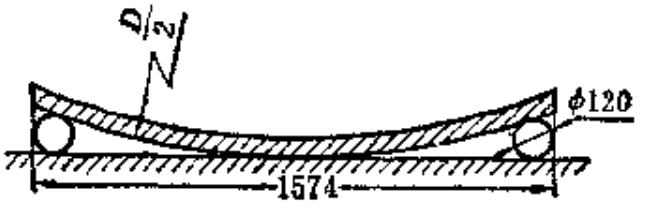
\includegraphics[width=7cm]{../pic/czjh2-ch7-fuxi-21.png}
    \caption*{(第 21 题)}
\end{figure}

\xiaoti{半径为 $R$ 和 $r$ ($R > r$) 的两圆相外切。求一条外公切线的长。}

\xiaoti{画出图中由圆和弧所组成的图案。}

\begin{figure}[htbp]
    \centering
    \begin{minipage}[b]{4cm}
        \centering
        \begin{tikzpicture}
    \pgfmathsetmacro{\R}{1.5}
    \pgfmathsetmacro{\r}{\R/2}

    \tkzDefPoints{0/0/O}
    \tkzDefPoint(180:\R){A}
    \tkzDefPoint(0:\R){B}
    \tkzDefPoint(180:\r){O_1}
    \tkzDefPoint(0:\r){O_2}

    \tkzDrawCircle[thick](O,A)
    \tkzDrawArc(O_1,O)(A)
    \tkzDrawArc(O_2,O)(B)
    \tkzDrawSegment[dashed](A,B)
\end{tikzpicture}


        \caption*{甲}
    \end{minipage}
    \begin{minipage}[b]{4cm}
        \centering
        \begin{tikzpicture} % 复杂
    \pgfmathsetmacro{\R}{1}

    \tkzDefPoints{0/0/O}
    \tkzDefPoint(0:\R){A}
    \tkzDefRegPolygon[center,sides=4,name=P](O,A)
    \tkzCalcLength(P1,P2)  \tkzGetLength{PP}
    \tkzInterCC[R](P1,\PP)(P2,\PP)  \tkzGetSecondPoint{B}
    \tkzDefRegPolygon[center,sides=4,name=Q](O,B)
    % \tkzLabelPoints[centered](P1,P...,P4)
    % \tkzLabelPoints[centered](Q1,Q...,Q4)

    \tkzDrawCircle[thick](O,A)
    \tkzDrawSegments[dashed](P1,P3  P2,P4)

    \foreach \i in {1,...,4} {
        \ifnum\i=4\relax
            \pgfmathsetmacro{\n}{1}
        \else
            \pgfmathsetmacro{\n}{int(\i+1)}
        \fi

        \tkzDrawArc[R with nodes](P\n,\PP)(P\i,Q\i)
        \tkzDrawArc[R with nodes](P\i,\PP)(Q\i,P\n)
    }
\end{tikzpicture}


        \caption*{乙}
    \end{minipage}
    \begin{minipage}[b]{4cm}
        \centering
        \begin{tikzpicture} % 复杂
    \pgfmathsetmacro{\R}{1.2}
    \pgfmathsetmacro{\RR}{sqrt(2)*\R}
    \pgfmathsetmacro{\r}{\RR/2}

    \tkzDefPoints{0/0/O}
    \tkzDefPoint(0:\R){A}
    \tkzDefRegPolygon[center,sides=4,name=P](O,A)
    \tkzDefPoint(45:\RR){B}
    \tkzDefRegPolygon[center,sides=4,name=Q](O,B)
    \tkzDefPoint(45:\r){C}
    \tkzDefRegPolygon[center,sides=4,name=O](O,C)
    % \tkzLabelPoints[centered](P1,P...,P4)
    % \tkzLabelPoints[centered](Q1,Q...,Q4)
    % \tkzLabelPoints[centered](O1,O...,O4)

    \tkzDrawSegments[dashed](P1,P3  P2,P4)
    \tkzDrawPolygon[dashed](Q1,Q...,Q4)

    \foreach \i in {1,...,4} {
        \ifnum\i=4\relax
            \pgfmathsetmacro{\n}{1}
        \else
            \pgfmathsetmacro{\n}{int(\i+1)}
        \fi

        \tkzDrawArc[R with nodes](O\i,\r)(P\i,P\n)
    }
\end{tikzpicture}


        \caption*{丙}
    \end{minipage}
    \begin{minipage}[b]{4cm}
        \centering
        \begin{tikzpicture} % 复杂
    \pgfmathsetmacro{\R}{1.5}
    \pgfmathsetmacro{\RR}{sqrt(2)*\R}
    \pgfmathsetmacro{\r}{\RR/2}

    \tkzDefPoints{0/0/O}
    \tkzDefPoint(0:\R){A}
    \tkzDefRegPolygon[center,sides=4,name=P](O,A)
    \tkzDefPoint(45:\RR){B}
    \tkzDefRegPolygon[center,sides=4,name=Q](O,B)
    \tkzDefPoint(45:\r){C}
    \tkzDefRegPolygon[center,sides=4,name=O](O,C)
    % \tkzLabelPoints[centered](P1,P...,P4)
    % \tkzLabelPoints[centered](Q1,Q...,Q4)
    % \tkzLabelPoints[centered](O1,O...,O4)
    % \tkzLabelPoints[centered](O)

    \tkzDrawPolygon[dashed](Q1,Q...,Q4)
    % \tkzDrawPolygon[dashed](P1,P...,P4)
    % \tkzDrawPolygon[dashed](O1,O...,O4)

    \foreach \i in {1,...,4} {
        \ifnum\i=4\relax
            \pgfmathsetmacro{\n}{1}
        \else
            \pgfmathsetmacro{\n}{int(\i+1)}
        \fi

        \tkzDrawArc[](P\n,Q\n)(Q\i)
    }

    \foreach \i in {1,...,4} {
        \ifnum\i=4\relax
            \pgfmathsetmacro{\n}{1}
        \else
            \pgfmathsetmacro{\n}{int(\i+1)}
        \fi

        \begin{scope}
            \tkzClipPolygon[out](O,P\i,Q\i,P\n)
            \tkzDrawArc[fill=white](O\i,P\n)(P\i)
        \end{scope}
    }
\end{tikzpicture}


        \caption*{丁}
    \end{minipage}
    \caption*{(第 23 题)}
\end{figure}


\xiaoti{正十边形的边长为 $2a$, 求它的面积(用代数式表示)。}

\xiaoti{我国民间相传有正五边形的近似作法。“九五顶五九,八五分两边”,它的意义如图所示。}
\begin{xiaoxiaotis}

    \xxt{用这个方法作边长为 50 毫米的近似正五边形;}

    \xxt{用三角函数计算边长为 10 寸的正五边形中,相当于图中 5.9 寸、9.5 寸、8 寸的线段的长,加以比较。}

\end{xiaoxiaotis}

\begin{figure}[htbp]
    \centering
    \begin{minipage}[b]{7cm}
        \centering
        \begin{tikzpicture}
    \pgfmathsetmacro{\factor}{0.25}

    \tkzDefPoint(0,0){O}
    \tkzDefPoint(5*\factor,0){A}
    \tkzDefPoint(8*\factor,9.5*\factor){B}
    \tkzDefPoint(0,(9.5+5.9)*\factor){C}
    \tkzDefPoint(-8*\factor,9.5*\factor){D}
    \tkzDefPoint(-5*\factor,0){E}
    \tkzDefPoint(0,9.5*\factor){F}
    % \tkzLabelPoints[centered](A,...,F,O)

    \tkzDrawPolygon(A,...,E)
    \tkzDrawSegments(B,D  O,C)
    \tkzLabelSegment[above, sloped](O,F){9.5寸}
    \tkzLabelSegment[pos=.4, above, sloped](F,C){5.9寸}
    \tkzLabelSegment[below](F,B){8寸}
    \tkzLabelSegment[below](F,D){8寸}
    \tkzLabelSegment[below](O,A){5寸}
    \tkzLabelSegment[below](O,E){5寸}
\end{tikzpicture}


        \caption*{(第 25 题)}
    \end{minipage}
    \qquad
    \begin{minipage}[b]{7cm}
        \centering
        \begin{tikzpicture}
    \pgfmathsetmacro{\R}{3}
    \pgfmathsetmacro{\r}{2}

    \tkzDefPoint(0,0){O}
    \tkzDefPoint(130:\R){A}
    \tkzDefPoint(130:\r){A'}
    \tkzDefPoint(60:\R){B}
    \tkzDefPoint(60:\r){B'}

    \tkzFillSector[pattern={mylines[angle=45, distance={3pt}]}](O,B)(A)
    \tkzFillSector[fill=white](O,B')(A')
    \tkzDrawSector[thick](O,B)(A)
    \tkzDrawArc[thick](O,B')(A')
    \tkzLabelArc[above](O,B,A){$l$}
    \tkzLabelArc[below](O,B',A'){$l'$}
    \tkzLabelSegment[centered, rotate=40, xshift=-.6em](A,A'){$d$}
    \tkzLabelPoints[below](O)
    \tkzLabelPoints[below left](A,A')
    \tkzLabelPoints[right](B,B')
\end{tikzpicture}


        \caption*{(第 29 题)}
    \end{minipage}
\end{figure}

\xiaoti{求证:两个同心圆所成环形的面积等于以切于小圆的大圆的弦为直径的圆的面积。}

\xiaoti{半径为 $R$ 的两个等圆互相经过圆心,求两圆所围的公共部分的面积。}

\xiaoti{已知:直角三角形 $ABC$ 及斜边 $BC$ 上的高 $AD$。
    求证: $\triangle ABD$ 和 $\triangle ACD$ 的内切圆的面积的比等于 $BD:DC$。
}

\xiaoti{如图, $\yuanhu{AB}$ 与 $\yuanhu{A'B'}$ 的圆心都是 $O$,
    $AA' = d$, $\yuanhu{AB}$ 的长是 $l$, $\yuanhu{A'B'}$ 的长是 $l'$。求证:
}
\begin{xiaoxiaotis}

    \xxt{$\angle O = \dfrac{l - l'}{d} \times \dfrac{180}{\pi}$ 度;}

    \xxt{$S_{AA'B'B} = \exdfrac{1}{2} (l + l') \, d$。}
\end{xiaoxiaotis}

\xiaoti{如图, $B$ 是 $AC$ 上的一点, 分别以 $AB$、$BC$、$AC$ 为直径作半圆。
    从 $B$ 作 $BD \perp AC$, 与半圆相交于 $D$。
    求证:图中阴影部分的面积等于以BD为直径的圆的面积。
}

\begin{figure}[htbp]
    \centering
    \begin{minipage}[b]{7cm}
        \centering
        \begin{tikzpicture}
    \tkzDefPoints{0/0/A, 4/0/C}
    \tkzDefPointOnLine[pos=0.4](A,C)  \tkzGetPoint{B}
    \tkzDefMidPoint(A,C)  \tkzGetPoint{O}
    \tkzDefMidPoint(A,B)  \tkzGetPoint{O1}
    \tkzDefMidPoint(B,C)  \tkzGetPoint{O2}
    \tkzDefLine[perpendicular=through B](A,C)  \tkzGetPoint{d}
    \tkzInterLC(B,d)(O,A)  \tkzGetFirstPoint{D}
    \tkzDefMidPoint(B,D)  \tkzGetPoint{O3}

    \tkzFillSector[pattern={mylines[angle=45, distance={3pt}]}](O,C)(A)
    \tkzFillSector[fill=white](O1,B)(A)
    \tkzFillSector[fill=white](O2,C)(B)
    \tkzDrawArc[thick](O,C)(A)
    \tkzDrawArc[thick](O1,B)(A)
    \tkzDrawArc[thick](O2,C)(B)
    \tkzDrawCircle[very thick](O3,B)
    \tkzDrawSegments[thick](A,C  B,D)
    \tkzLabelPoints[below](A,B,C)
    \tkzLabelPoints[above](D)
\end{tikzpicture}


        \caption*{(第 30 题)}
    \end{minipage}
    \qquad
    \begin{minipage}[b]{7cm}
        \centering
        \begin{tikzpicture}
    \pgfmathsetmacro{\factor}{0.1}

    % 坐标
    \tkzDefPoints{-15*\factor/0/x1, 50*\factor/0/x2, 0/-15*\factor/y1, 0/22*\factor/y2}
    \tkzDrawSegments[-|Latex](x1,x2  y1,y2)
    \tkzLabelSegment[pos=1, below](x1,x2){$x$}
    \tkzLabelSegment[pos=1, left](y1,y2){$y$}

    % 圆 O
    \pgfmathsetmacro{\Ra}{10*\factor}
    \tkzDefPoint(0,0){O}
    \tkzDefPoint(100:\Ra){L}
    \tkzDrawCircle[thick](O,L)
    \tkzDrawSegment[-Latex](O,L)
    \tkzLabelSegment[pos=.3, left](O,L){$R10$}
    \tkzLabelPoints[below left](O)

    % 圆 O_1
    \pgfmathsetmacro{\Rb}{8*\factor}
    \tkzDefPoint(35*\factor,0){O_1}
    \tkzDefShiftPoint[O_1](100:\Rb){M}
    \tkzDrawCircle[thick](O_1,M)
    \tkzDrawSegment[-Latex](O_1,M)
    \tkzLabelSegment[right=-.2em](O_1,M){$R8$}
    \tkzLabelPoints[below](O_1)


    % 点 P 及弧线
    \pgfmathsetmacro{\Rc}{27*\factor}
    \tkzDefPoint(31.90*\factor,18.75*\factor){P}
    \tkzDefShiftPoint[P](240:\Rc){N}
    \tkzInterLC[R](O,P)(O,\Ra)  \tkzGetSecondPoint{A}
    \tkzInterLC[R](O_1,P)(O_1,\Rb)  \tkzGetSecondPoint{B}
    \tkzDrawArc[dashed](P,A)(B)
    \tkzDrawSegment[-Latex](P,N)
    \tkzLabelSegment[above, sloped](P,N){$R27$}
    \tkzDrawPoint(P)
    \tkzLabelPoints[right](A)
    \tkzLabelPoints[below](B)
    \tkzLabelPoint[right](P){$P(x,y)$}
\end{tikzpicture}


        \caption*{(第 35 题)}
    \end{minipage}
\end{figure}

\xiaoti{}%
\begin{xiaoxiaotis}%
    \xxt[\xxtsep]{举出原命题和逆命题都正确以及原命题正确而逆命题不正确的例子;}

    \xxt{举出原命题和否命题都正确以及原命题正确而否命题不正确的例子;}

    \xxt{能不能举出原命题正确而逆否命题不正确的例子?为什么?}

\end{xiaoxiaotis}

\xiaoti{图形 $F$ 是符合条件 $C$ 的点的轨迹,需要下列两个命题都正确:
    1. 图形 $F$ 上的每一个点都符合条件 $C$;
    2. 符合条件 $C$ 的每一个点都在图形 $F$ 上。
}
\begin{xiaoxiaotis}

    \xxt{如果命题 1 正确,命题 2 不正确,会发生什么情况?举例说明;}

    \xxt{如果命题 1 不正确,命题 2 正确,会发生什么情况?举例说明。}
\end{xiaoxiaotis}

\xiaoti{已知 $\yuan\,O$ 上一点 $A$,说明并作出以点 $A$ 为端点的弦的中点的轨迹(不要求证明)。}

\xiaoti{求作一个圆,使它的半径等于 3 cm, 经过已知点 $A$,并且和半径为 2 cm 的已知圆 $O$ 相切(已知 $OA = 6$ cm)。}

\xiaoti{在如图所示的坐标系中, $\yuan\,O$ 的半径为 10, $O_1 $的坐标为 $(35, 0)$,
    $\yuan\,O_1$ 的半径为 8。 $\yuanhu{AB}$ 与 $\yuan\,O$ 上的弧外连接,
    与 $\yuan\,O_1$ 上的弧内连接。计算 $\yuanhu{AB}$ 所在圆的圆心 $P$ 的坐标(保留4个有效数字)。
}


\end{enhancedline}
\end{xiaotis}

